
\newcommand{\rc}{R_c}
\newcommand{\Calorif}{\mbox{\large$\mathbf{c}$}}
\newcommand{\rp}{R_p}
\newcommand{\grad}{$^\circ$}
\newcommand{\Fp}{F_P}
\newcommand{\Peff}{P}
\newcommand{\ideal}{{ideal}}
\newcommand{\perd}{{perd.}}
\newcommand{\Pideal}{P_\ideal}
\newcommand{\Pperd}{P_\perd}
\newcommand{\Pind}{P_i}
\newcommand{\pmi}{p_{mi}}
\newcommand{\Pot}{{ \mbox{\tiny$P$}}}
\newcommand{\Potmax}{{ \mbox{\tiny$P_\max$}}}
\newcommand{\Torq}{{ \mbox{\tiny$T$}}}
\newcommand{\Torqmax}{{ \mbox{\tiny$T_\max$}}}
\newcommand{\Ce}{C_e}
\newcommand{\pme}{p_{me}}
\newcommand{\etaeff}{\eta_{total}}
\newcommand{\etavol}{\eta_{{\mbox{\tiny$V$}}}}
\newcommand{\util}{\acute{u}til}

\renewcommand{\min}{{m\textrm{í}n}}
\renewcommand{\max}{{m\acute{a}x}}
\newcommand{\ctegas}{k}
\newcommand{\rv}{{R_{\mbox{\tiny $V$}}}}
 \mathchardef\mhyphen="2D
 \newcommand{\hyph}{\,\mhyphen}
 \vspace{.9cm}
{\centering 
{\bf \LARGE Primer Parcial \par}
}
\begin{center}
\vspace{-.2cm}\rule{3cm}{2pt}\par
\vspace{-.2cm}
\end{center}
\part{Introducción}
\section{Que son estas cosas?}

Un motor térmico es cualquier dispositivo que puede quemar una mezcla de aire y combustible en una cámara de combustión (interna o externa) y convertir dicha energía térmica en energía mecánica.

\begin{itemize}
    \item {\bf Motores a combustión interna o endotérmicos:} El cambio térmico se genera en el mismo fluido de trabajo en el interior del motor.
    \item {\bf Motores de combustión externa o exotérmicos:} Al fluido de trabajo se le transmite el estado térmico a través de una pared (como una turbina).
    \begin{itemize}
        \item Fueron usados extensivamente durante la revolución industrial.
        \item Rendimiento bajo y alta contaminación.
    \end{itemize}
\end{itemize}

Tipo de motor endotérmico (MCI):
\begin{itemize}
    \item \textbf{MEP}: Motores de encendido provocado.
    \item \textbf{MEC}: Motores de encendido por compresión.
\end{itemize}

El funcionamiento de un motor MCI se rige por el movimiento de su cigüeñal. Este marca el ritmo al cual empiezan y terminan los ciclos dentro del pistón. Es importante saber que el cada ciclo de combustión son 2 vueltas del cigüeñal para un motor de 4 tiempos (el más común). 

Motores ciclo Otto son encendidos a chispa mientras que los motores a ciclo Diesel se encienden por compresión. La diferencia principal entre estos motores es que el calor aportado en el Otto idealizado ocurre a volumen constante (en un instante) mientras que en el Diesel el calor es aportado a presión constante. 

{\bf Potencia en motores.} Si quiero más potencia en un \textbf{Otto} entrego más \textit{aire y combustible}. Si quiero hacer lo mismo en un \textbf{Diesel} entrego más \textit{combustible}. La eficiencia térmica en motores está dada por:

\[
\eta_t=\frac{W_{\util}}{Q_{entregado}}=\frac{Q_{entregado}-Q_{perdido}}{Q_{entregado}}=1-\frac{Q_{perd}}{Q_{entr}}
\]
Para un Otto esto vale:
\[
\eta_{t_{Otto}}=1-\frac{1}{\ctegas}\frac{T_4-T_1}{T_3-T_2}
\]
\section{Motores Otto}

\textbf{El combustible nafta o gasolina.} 
\begin{itemize}
    \item Mezcla pobre es preferible por razones de contaminación 
    \item Mezcla estequiométrica:\textit{Aire a gasolina} \textbf{14,7:1} (masa) 
    \begin{itemize}
        \item Reducir esta relación (mezcla más rica) aumenta contaminación y crea humo negro (material particulado) y otros problemas
    \end{itemize}
    \item Densidad \textbf{0,71-0,76 kg/lt} con un poder calorífico de $\Calorif_{nafta}\cong$ \textbf{44.000 kJ/kg}
\end{itemize}

\textbf{Características del motor Otto.}
El ciclo se mide en angulo transversado del cigüeñal. Un ciclo, tanto para motor Otto como Diesel, tiene 720$^\circ$. 
\begin{itemize}
\item Encendido logrado con un arco eléctrico con bujías
\item Inyector de combustible puede estar dentro de la conjunto pistón (inyección directa) o en el trayecto de admisión (inyección indirecta). Diesel solo adentro de la cámara.
\item Mayor contenido de $CO$ monoxido de carbono en los gases de escape comparado al Diesel.
\item Los motores Otto de la actualidad regulan la potencia controlando la relación Aire/Combustible mediante una mariposa de aceleración (control aire) y inyectores electrónicos (control combustible)
\item Presiones menores a las del Diesel en general
\item Rendimiento térmico superior al Diesel Mixto pero menor que el Diesel.
\item Comparado a Diesel grado de compresión bajo. $\rc = 8\,\mhyphen 11$ con presión $p_{compresi\acute{o}n}=13\,\mhyphen15\, bar$ y $p_\max=30\,\mhyphen40\,bar$.
\end{itemize}
\subsection{Etapas del ciclo}

\begin{itemize}
    \item {\bf Admisión}
    \begin{itemize}
        \item El pistón desciende desde el \textbf{Punto Muerto Superior} (PMS) al \textbf{Punto Muerto Inferior} (PMI). Válvula de admisión abierta y la de escape cerrada
    \end{itemize}
    \item \textbf{Compresión}
    \begin{itemize}
        \item Se cierra la válvula de admisión y sube el pistón al PMS con ambas valvulas cerradas. $p_f=10-15\,bar$
    \end{itemize}
    \item  \textbf{Expansión}
    \begin{itemize}
        \item Se produce la chispa y por ende la combustión antes del PMS. Durante la expansión el pistón desciende del PMS al PMI produciéndose el trabajo útil
    \end{itemize}
    \item \textbf{Escape}
    \begin{itemize}
        \item El pistón sube del PMI al PMS con la válvula de escape abierta extrayéndose los gases de combustión
        \item El ciclo se vuelve a repetir en estos 4 pasos
    \end{itemize}
\end{itemize}
\textbf{Ciclo ideal.} En el ciclo ideal cada etapa es de 180$^\circ$ del cigüeñal. Todas sumadas dan 720$^\circ$.

\textbf{Ciclo real.} El ciclo real \textbf{todas} las etapas son más largas que sus contrapartes ideales a causa del avance y retraso de cierre de las válvulas de escape y admisión. La suma de todas las etapas \textit{reales} da más de 720$^\circ$. \footnote{Se suele decir que el \textbf{ciclo} tiene más de 720$^\circ$, aunque es un concepto erróneo ya que un \textbf{ciclo} por definición comienza y termina en el mismo lugar.}

\begin{itemize}
    \item \textbf{AAA:} Avance a la apertura de la válvula de admisión
    \item \textbf{AAE:} Avance a la apertura de la válvula de escape
    \begin{itemize}
        \item La valvula de escape se abre antes del PMI para aprovechar presión remanente de la combustión y así vaciar el cilindro de gases de combustión
    \end{itemize}
    \item \textbf{RCE:} Retraso al cierre de la válvula de escape
    \item \textbf{RCA:} Retraso al cierre de la válvula de admisión
    \item \textbf{AE:} Avance de encendido
    \begin{itemize}
        \item Varía entre $5^\circ-40^\circ$
    \end{itemize}
    \item \textbf{CV=AAA+RCE:} Cruce de válvulas
\end{itemize}
\subsubsection{Diagrama Polar}
Estudiar esto
\subsection{Relación de compresión}
Se tiene el volumen unitario $V_u$, definido como el volumen que ``barre'' el pistón en su recorrido. El volumen de cámara de combustión es el volumen \textit{mínimo} alcanzado durante la combustión. $V$ es el volumen total o cilindrada, equivalente al volumen unitario multiplicado por cantidad de cilindros: $V=V_u\cdot N$

\[
\rc=\frac{V_u+V_c}{V_c}
\]
$\rc$ es la relación de compresión del motor la cual define varias eficiencias.

Si se considera el gas de la cámara como ideal se puede definir el \textbf{rendimiento térmico del Otto} como

\[
\eta_t=1-\frac{1}{\rc^{\ctegas-1}}=1-\left(\frac{V_\min}{V_\max}\right)^{\ctegas-1}
\]
donde $\ctegas=\frac{c_p}{c_v}\approx1,33$ para Otto.

\textbf{Cruce de válvulas.} Se produce con la apertura simultanea de las válvulas de admisión y escape al fin de la etapa del escape. Esto permite que aún con el pistón detenido en el PMS los gases circulen gracias a su inercia, trayendo aire fresco. La apertura del la válvula de escape también ayuda a reducir la presión en el cilindro favoreciendo la entrada de aire por la adimisión. Esto refrigera el cilindro y aumenta la concentración de aire para el próximo ciclo. 

A medida que aumenta el número de vueltas (la velocidad [rpm del cigüeñal]) el tiempo de intercambio de gases se reduce. Por lo tanto se necesita aumentar el cruce de válvulas. Cuanto más rápido el motor$\Rightarrow$ Mayor cruce de válvula. Para motores Otto $CV=0-35^\circ$. Los motores grandes tienen un cruce de válvulas reducido.

\section{Motor Diesel}

\textbf{El combustible Diesel o gasóleo.} 
\begin{itemize}
    \item Siempre funciona a exceso de aire, es decir, los motores Diesel regulan la potencia mediante el control del combustible inyectado (no hay mariposa!)
    \item Mezcla estequiométrica: \textit{Aire a gasóleo} \textbf{14,5:1} (masa)
    \begin{itemize}
        \item Reducir esta relación (mezcla más rica) aumenta contaminación y crea humo negro (material particulado) y otros problemas
    \end{itemize}
    \item Densidad \textbf{0,81-0,85 kg/lt a }$15^\circ C$ con un poder calorífico de $\Calorif_{Diesel}\cong$ \textbf{42.000 kJ/kg}
    \item Viscosidad aumenta violentamente con descenso de temperatura. Se necesita un precalentador para $T\lesssim-25^\circ$
    \item Combustible tiene un \textbf{retraso de ignición} o \textbf{encendido} entre inyección y comienzo del frente de llama
    \item Presión de combustión entre 70-90 bar y se requiere una temperatura elevada T>500\grad.
\end{itemize}
Como bien se menciono anteriormente, la potencia es otorgada por un aumento de combustible, \textit{no hay cambio de cantidad de aire en la cámara}. Al acelerar se aumenta la cantidad de combustible y aumenta la potencia erogada por el motor.

\textbf{Método de inyección.}
Dos métodos principales para motores Diesel:
\begin{itemize}
    \item Motores de inyección directa (a la cámara de combustión)
    \begin{itemize}
        \item Mejor rendimiento térmico y especifico
        \item Requiere biela y cigüeñal robustos
        \item 99,9\% motores de este tipo
    \end{itemize}
    \item Motores de inyección ``indirecta'' lo hacen en una precámara de inyección
    \begin{itemize}
        \item Vibraciones mas suaves, mejor para autos pequeños
        \item Contamina más
    \end{itemize}
\end{itemize}

\textbf{Características de la preinyección en el Diesel.} Para motores chicos se efectúa una o multiples pre-inyecciones que con el tiempo llegan a homogenizarse en la cámara completamente y luego se enciende \textit{antes} de la inyección principal. Con esto se logra que la inyección principal caiga sobre un frente de llama, acelerando el proceso de combustión. Dicho esto, el retraso de tiempo de ignición se achica considerablemente.

{\bf Características del motor Diesel.}
\begin{itemize}
    \item No existe mariposa de aceleración
    \item Exceso de aire es deseable
    \item Aumento de temperatura de aire del ambiente afecta rendimiento negativamente\footnote{A mayor temperatura, menor densidad de aire $\Rightarrow$ menor masa de aire en cámara.}
    \item Bujías de \emph{precalentamiento}. Favorece arranque en frió
    \item Presiones mayores que en Otto. Componentes (biela, perno de pistón cigüeñal) reforzados
    \item Motores Diesel modernos en el rango de $\rc\approx 21$ y presión máxima alcanzada durante la combustión $p_{\max}\approx 190\,bar$, presión media efectiva $\pme\approx 25\, bar$ y presión de inyección (Common rail 3rd gen) $p_{iny}=2000\,\mhyphen 3000\, bar$
    \item \textbf{Diesel Lento:}Funcionamiento duro y ruidoso con alto tiempo de retraso. Inyectores de multiples orificios. Usados en camiones, locomotoras, barcos y generadores. Cilindradas mayor a 3300cm$^3$ 
    \item \textbf{Diesel Rápido:} Superan los 4500 rpm. Común usar camaras combustión integradas al pistón. Preinyecciones (3-10\% de inyección total) antes de inyección principal (ayudan que sea mas suave el funcionamiento). Cilindradas menores a 3500cm$^3$ 
\end{itemize}

{\bf Ciclo Diesel.} 

El rendimiento térmico en un ciclo Diesel \textbf{ideal} está dado por 
\[
\eta_t=\frac{W_{\util}}{Q_{entr.}}=1-\frac{1}{\rc^{\ctegas-1}}\left( \frac{\rv^\ctegas-1}{\ctegas(\rv-1)}\right)
\]
donde $\ctegas=\frac{c_p}{c_v}\approx1,4$ para Diesel, $\rv$ es la relación de cut-off $\frac{V_4}{V_3}$ (relación de volúmenes al comienzo y al final de la etapa de combustión).

Para un ciclo Diesel mixto o \textbf{ciclo Sabathé}

\[
\eta_t = 1- \frac{T_5-T_1}{(T_3-T_2)+\ctegas(T_4-T_3)}
\]
puede resultar útil también tener en cuenta la otra expresión
\[
\eta_t=1-\frac{1}{\rc^{\ctegas -1}}\cdot \frac{\rp(\rv)^\ctegas-1}{(\rp -1)+\ctegas\rp(\rv-1)}\]
donde $\rp=\frac{p_3}{p_2}$ es la relación de presiones en la parte a volumen constante (etapa semejante al ciclo Otto) y $\rv = \frac{V_5}{V_4}$.

\textbf{Combustión en el ciclo Diesel.} El combustible es inyectado antes del PMS (\textbf{AI}:Avance de inyección. \textbf{Reemplaza el concepto de AE en el Otto}). Esto le da tiempo para mezclarse al combustible. Es deseable alta temperatura, gran turbulencia  pulverización fina, buena cantidad de oxigeno para favorecer la combustión. Los últimos dos puntos favorecen la combustión completa, reduciendo PM (material particulado$\equiv$ contaminación) y aumentando la eficiencia. Cuidarse que a muy alta temperatura se forman óxidos de nitrógeno muy contaminantes!

Se puede reducir el \textbf{retraso de encendido} usando un combustible de número de cetano adecuado, alta turbulencia en la cámara, regulando caudal de inyección inicial y con preinyecciones antes de la inyección principal.

\textbf{Avance de inyección:} 
\begin{itemize}
    \item Compensa la propiedad intrínseca retraso de encendido del combustible Diesel
    \item Se desea que el pistón se encuentre en el PMS al final de la combustión
    \item Hoy en día se regula electrónicamente el avance de encendido dependiendo de variables de trabajo del motor
\end{itemize}

\textbf{Sobrealimentación (turbo-compresor) en Diesel.} Como el factor limitante a la potencia es el aire, se ideo un sistema que aumente la alimentación de aire a la cámara usando la energía cinética de los gases de escape. Funciona alrededor de 80-120 mil rpm.
\begin{itemize}
    \item Mejora rendimiento notablemente
    \item Aumentar rendimiento químico (se oxida un mayor porcentaje del combustible)
    \item Diesel lentos de cilindrada $V_u$ grande
    \begin{itemize}
        \item Mejora en intercambio de gases
        \item Proporciona el aire suficiente en altas cargas
    \end{itemize}
    \item Diesel rápidos con cilindradas chicas
    \begin{itemize}
        \item Interesa obtener una buena relación peso/potencia
        \item Se logra buen consumo y rendimiento
    \end{itemize}
    \item Se tiene que controlar la velocidad. Si aumenta la realimentación $\Rightarrow$ aumenta energía de gases de escape $\Rightarrow$ circulo vicioso. A esto se lo llama \textit{embalamiento}. Para prevenir esto existe la válvula de alivio que hace un cortocircuito entre trayecto de admisión y el escape.
\end{itemize}

\section{Comparación entre MEP y MEC}
\subsection{Ventajas e inconvenientes del Diesel respecto al Otto.}

\begin{itemize}
    \item Ventajas
    \begin{itemize}
        \item Mayor $\eta_t$ por temp. mayores
        \item Menor consumo
        \item Menor monoxido de carbono y hidrocarburos no quemados
    \end{itemize}
    \item Inconvenientes
    \begin{itemize}
        \item Mayor contaminación con óxidos de nitrógeno y dioxido de azufre
        \item A igual cilindrada son más robustos y por lo tanto más caros
        \item Mayor dificultad en arranque en frió
        \item Funcionamiento brusco
    \end{itemize}
\end{itemize}
Ver pg. 16 del Giacosa.

\section{Potencia y rendimiento}
Los factores que determinan el rendimiento del motor:
\begin{itemize}
    \item \textbf{Grado de compresión.} $\rc \uparrow$,$\eta \uparrow$. Limitado por detonación
    \item \textbf{Desarrollo de combustión.} Mezcla homogénea, frente de llama uniforme
    \item Relación A/C (aire-combustible)
\end{itemize}

\subsection{Potencias}
\textbf{La potencia ideal} $P_\ideal$ se obtiene del ciclo teórico y va relacionada con la presión media efectiva $W_\ideal = \pme V_u$. El rendimiento térmico es calculado para los ciclos ideales de tal forma que  
\[
\Pideal=\eta_t\cdot\Fp=\eta_t \cdot \dot{m}_c \Calorif
\]
también vale para motores de 4 tiempos: $\Pideal=\frac{N V_u \pme}{2}\cdot \frac{n}{60}$
donde $\Calorif$ es el poder calorifico del combustible.

\textbf{Potencia indicada} \textit{es la potencia desarrollada en el interior del cilindro}. Se obtiene a partir del ciclo real, siendo esta el área encerrada por la linea que recorre el ciclo en el gráfico $p$-$V$. La potencia indicada toma en cuenta el \textit{trabajo de bombeo}, $\ctegas=\frac{c_p}{c_v}$ no constante, las perdidas de calor al refrigerante entre varias otras cosas.
\[
P_i=P_\perd+\Peff
\]
donde $P_\perd$ es la potencia asociada con las perdidas mecánicas y $\Peff$ es la potencia efectiva, o la potencia útil.

Se define una nueva presión media, llamada la \textit{presión media indicada} $\pmi$. En un motor de \textbf{4 tiempos} que el ciclo se completa en 2 revoluciones:
\[
P_i = \frac{N V_u \cdot \pmi}{2}\cdot \frac{n}{60}
\]
donde $N$ es el número de cilindros y $n$ son las revoluciones en rpm.

\textbf{Potencia efectiva o útil.} También conocida como la potencia al freno porque se mide aplicando un dispositivo al eje del motor frenandolo y midiendo el par que genera a una velocidad $n$.
\[
\Peff=T\cdot \omega = T \cdot \frac{2\pi \cdot n}{60}=\Pind-\Pperd
\]
donde $T$ es el par y $\omega$ es la velocidad en radianes por segundo. Resultado en [W].
\subsection{Rendimientos}
\textbf{Rendimiento térmico.} Definido de otra manera
\[
\eta_t=\frac{\Pideal}{\dot{m}_c \Calorif}=\frac{\Pideal}{\Fp}
\]
donde $\dot{m}_c$ es caudal másico de combustible quemado y $\Calorif$ es el poder calorífico del combustible. $\Fp=\Calorif \dot{m}$ es el \emph{fuel power.} El limitante al rendimiento térmico son las temperaturas. Si se supera cierto valor hay riesgo de autoignición de la mezcla.

Otto: $\eta_t=35\,\mhyphen40\%$

Diesel: $\eta_t=40\,\mhyphen50\%$


\textbf{Rendimiento indicado.} Es la relación entre el trabajo del ciclo indicado y el trabajo del ciclo ideal.

\[\eta_i=\frac{P_i}{P_\ideal}\]
donde $P_i=P+P_{perdidas}$.


\textbf{Rendimiento mecánico.} Relación entre la potencia efectiva que se obtiene en el eje del motor y la potencia indicada que se obtiene en el diagrama de trabajo real del motor en el cual no intervienen las perdidas mecánicas.

\begin{itemize}
    \item Hay perdidas debido al rozamiento entre aros del pistón, camisa y perdidas a la fricción del lubricante entre otras.
    \item Energía consumida en dispositivos auxiliares como bombas
\end{itemize}

\[
\eta_m = \frac{\Peff}{P_i}
\]
en general ronda $\eta_m=85\hyph90\%$.


\textbf{Rendimiento efectivo (o total).} La relación entre las perdidas totales del motor y la energía contenida en el combustible consumido definen el rendimiento efectivo del motor.

Otto: $\etaeff=25\hyph30\%$

Diesel: $\etaeff = 30\hyph 40\%$

\[
\etaeff=\frac{P_{\ideal}}{\Fp}\cdot\frac{P_i}{P_\ideal}\cdot \frac{P}{P_i}=\eta_t\cdot \eta_i \cdot \eta_m = \frac{\Peff}{\Fp}
\]

\textbf{Rendimiento volumétrico.} Se puede definir como el grado de eficiencia con el que se introduce la carga fresca al cilindro o grado de llenado.

\textit{Es la relación entre la masa de aire introducida al cilindro y la masa de aire teórica necesaria para llenar el cilindro calculada en base a las dimensiones del cilindro y condiciones atmosféricas} $(p,T)$.

\[
\etavol = \frac{M_{aire}}{M_{aire\textrm{ }\ideal }}
\]

Dicho rendimiento depende del régimen de giro, condiciones ambientales, sección de válvulas (agregar válvulas mejora el rendimiento), perdidas en la admisión y la eficacia de barrido de gases.

\subsection[Como mejorar rendimiento volumétrico]{Como mejorar $\etavol$}
\begin{itemize}
    \item Se pueden reducir las pérdidas en el conducto de admisión
    \item Agregar un turbocompresor
    \item Ajustar el cruce de valvulas para el régimen de funcionamiento ($n$)
    \item Bajar la temperatura a la cual ingresa el aire en la admision
    \item Aumentar válvulas por cilindro. Es preferible 2 válvulas de admisión ante 1 debido a la inercia del aire
    \item $\etavol$ es mínima en ralentí y al máximo numero de vueltas.
\end{itemize}


\section{Parámetros característicos} 


\textbf{Presión media efectiva.} La presión durante la combustión no es constante pero resulta útil obtener un parámetro representativo de ella. La $\pme$ resulta de hallar la presión media durante el tiempo de combustión y expansión. 

\[
\pme \approx \frac{W_{\text{comb-exp}}}{V_u}
\]
esta presión caracteriza el par desarrollado del motor. Depende principalmente del grado de llenado de los cilindros, la eficacia de la combustión y el régimen del motor (mayor en $n_{{\etavol}_{\max}}$).

\textbf{Potencia motor o potencia al freno.} 
\[
P=T\omega=T \cdot 2 \pi f = T \frac{2\pi n}{60}
\]
donde $n$ son las revoluciones [rpm], y $T$ es el torque o par [Nm]. Resultado en [W]. Lo que determina la potencia esta dado en gran parte por la cilindrada $V_u$, $\etavol$, $\rc$ y $n$.

\[
1\, HP \approx 745,7\, W
\]

Esta potencia también se conoce como potencia al freno o \textit{brake power} porque se obtiene en un ensayo donde se calcula la potencia frenando el motor y midiendo las vueltas y el par.

\textbf{Factores que determinan la potencia de un motor.}

\begin{itemize}
    \item Cilindrada
    \item Grado de llenado de cilindros ($\etavol$)
    \item Relación de compresión
    \item Régimen de giro
\end{itemize}

\textbf{Consumo especifico de combustible.} $\Ce$ expresa relación entre masa combustible consumida y potencia. Depende principalmente de $\eta_t$ y $\etavol$. Por lo general el mínimo $\Ce$ se obtiene en la zona de par máximo (o cercanía), que coincide con el máximo $\etavol$ y máximo $\pme$. $\Ce$ esta en función de $\etavol$ que a la vez esta en función de las rpm, por ende $\Ce$ depende de las rpm.

\[
\Ce = \frac{\dot{m}_c}{P}
\]

Para Otto varía entre 280-320 g/kWh y para Diesel 180-280 g/kWh (mejor).

\textbf{Elasticidad de motor.} El campo de elasticidad $E$ se define como la diferencia de velocidad a alto régimen y a bajo/medio régimen. Un motor más elástico es mas ``cómodo'' de manejar debido a que hay que rebajar menos cantidad de veces al cambiar de revoluciones que con un motor menos elástico. 

\[
E = n_{\Potmax}-n_{\Torq_{\max}}
\]
si se va comparar el motor con un motor de otro rubro se puede efectuar una ponderación $E_{pond}=\frac{E}{n_{\max}}$.

El coeficiente de elasticidad está dado por
\[
E_c=E_n\cdot E_\Pot = \frac{n_{\Potmax}}{n_{\Torq_\max}} \cdot \frac{T_{\max}}{T_{\Potmax}}
\]
donde $E_n$ es la elasticidad de régimen y $E_p$ es la elasticidad de par. $T$ es el par (en N.m).

\begin{figure}
    \centering
    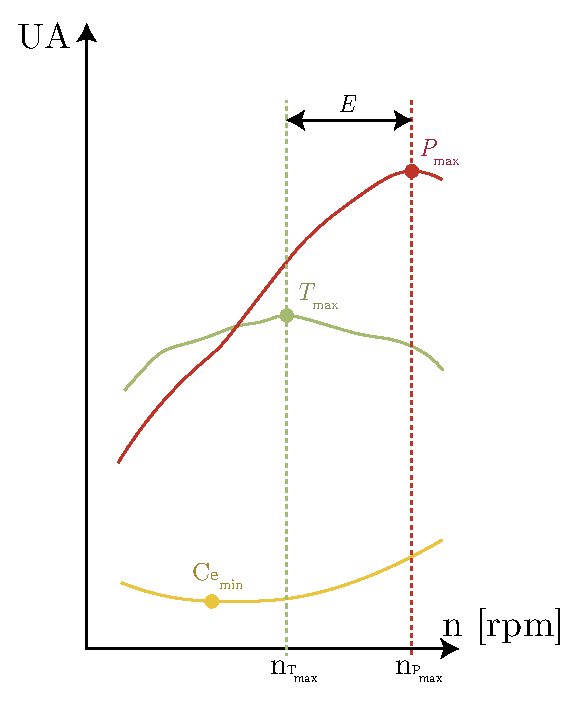
\includegraphics[width=.47\textwidth]{fig/curvaCaract.eps}
    \caption{Curvas características de un motor}
    \label{fig:curvacaract}
\end{figure}
\textbf{Consideraciones del ensayo.} Al realizar los ensayos para obtener los parámetros anteriores es muy importante tomar en cuenta las condiciones atmosfericas ya que $\etavol$ depende de estas y por lo tanto también la potencia. Se tiene que tomar en cuenta $p_{amb}$, $T_{amb}$ y en algunos casos humedad relativa $\phi_{amb}$.
\section{Disposición de cilindros}
Para motores de 4 tiempos ($720^\circ$ el ciclo completo) de $N$ cilindros se cálcula el ángulo por impulso: $\gamma_{imp} = \frac{720^\circ}{N}$.

Se comienzan a numerar los cilindros desde el lado opuesto de la salida de la transmisión y comenzando en la esquina inferior izquierda (mirando el motor de arriba con la transmisión saliendo para arriba).

Si se tiene un numero impar de pistones se tiene que usar un eje contrarrotante para contrarrestar las fuerzas no balanceadas que aparecen. Cada eje contrarrotante ejerce mitad de la fuerza de la biela, por ende se necesitan dos ejes contrarrotantes. (?)




\part{Dispositivos de motor}

\section{Resumen de dispositivos}
\subsection{Block de motor y otros elementos que lo acompañan}
\begin{itemize}
\item \textbf{Block de motor}
\begin{itemize}
\item Alberga cilindros/camisas
\item Fabricado de hierro (resistencia mecánica) o aleación ligera Al-Si (conductividad térmica, más ligero)
\item Puede tener sistema de refrigeración para refrigerar las camisas a base de liquido(más usado en actualidad) o aire
\item Constituye la estructura básica que soporta todos los componentes y demás elementos del motor
\item Debe ser rígido para permitir esfuerzos sin deformaciones, permitir canalizaciones de aceite/liquido refrigerante,  parte superior totalmente plana para sellado contra culata
\end{itemize}
\item \textbf{Tapa de cilindros} o \textbf{Culata}
\begin{itemize}
\item Cierra la parte superior de los cilindros. La superficie de asentamiento está rectificada para garantizar estanqueidad
\item Hechos de aluminio en la actualidad. Excelente conductividad térmica, buenas propiedades mecánicas y poco peso aunque es propensa a deformaciones. El hierro resiste deformaciones pero es más pesado.
\item Lleva orificios de refrigeración y conforma la parte superior de la cámara de combustión. Se puede refrigerar internamente por liquido (más común) o por aire mediante aletas. 
\item Contiene el árbol de levas, bujías, inyectores, balancines y válvulas
\end{itemize}
\item \textbf{Junta de culata}
\begin{itemize}
\item Encargada de que la unión entre bloque y tapa sea estanca
\item Pueden ser de dos tipos, multilaminares/multimetalicas o convencionales de fibra
\item Para motores Diesel se necesita determinar la saliente sobre el bloque del pistón para elegir una junta
\item Debe evitar fugas de compresión/liquido refrigerate/lubricante a altas temperaturas
\item Juntas multilaminares o multimetalicas son las más usadas y tienen entre 1 y 3 muescas que indican el saliente del pistón para motores Diesel
\end{itemize}
\item Bancadas o asientos de cigüeñal
\begin{itemize}
\item Donde apoyan los bujes de fricción que a su vez son el apoyo del cigüeñal del motor
\item Están recubiertos con un material más suave que el interior para atrapar metal o partículas disueltas en el lubricante
\end{itemize}
\item Semicárter
\item \textbf{Colectores de admisión}
\begin{itemize}
\item Objetivo es conducir el gas de admisión hacia los cilindros. Motores Otto de inyección indirecta tienen los inyectores montados dentro y existen diferentes tipos para este ultimo como \textit{monopunto, multipunto.}
\item Su forma tiene gran influencia en el $\etavol$.  Conduce gases del múltiple de admisión hacia la válvula de admisión
\item Pueden montarse en este tipo de conductos sistemas de admisión variable para adaptar las longitudes de los conductos a cada situación de funcionamiento de motor en cada caso.
\item Generalmente fabricados de aleación de aluminio
\end{itemize}
\item \textbf{Colector de escape}
\begin{itemize}
\item Conduce gases de escape hacia el silenciador de escape. Se suele hacer de fundición de hierro/acero inox. para soportar los grandes cambios de temperatura
\item Diseñado de tal forma para que las ondas de presión de cada cilindro no interfieran entre sí
\item Junta de unión con la culata soporta grandes temperaturas
\end{itemize}
\item \textbf{Sistema de escape}
\begin{itemize}
    \item Objetivo de conducir los gases a la atmósfera reduciendo su ruido y la contaminación mediante \textbf{silenciadores} y \textbf{catalizadores}, respectivamente.
\end{itemize}
\end{itemize}

\subsection{Otros componentes del motor}
\begin{itemize}
\item \textbf{Cigüeñal}
\item Sistema de distribución
\begin{itemize}
\item Comprende todos los elementos necesarios para coordinar la apertura y cierre de válvulas con el giro del motor
\item El cigüeñal arrastra el \textbf{árbol de levas} que a su vez controla las \textbf{válvulas} que actuan a través de la \textbf{guía de válvulas}
\item Resortes o muelles de válvulas
\item Taques y balancines
\end{itemize}
\item \textbf{Volante de inercia}
\begin{itemize}
\item Está engranado porque está acoplado al piñón del burro de arranque que pone el motor en marcha
\item Suaviza el andar del motor
\end{itemize}
\item Conjunto \textbf{Pistón}
\begin{itemize}
\item Camisa
\item Perno o bulón de pistón
\item Biela
\item Émbolo
\item Cámara
\item Bujes de biela
\item Aros de pistón
\end{itemize}
\end{itemize}
\section{Cámaras de combustión}
La cámara es conformada por la culata y el émbolo del pistón cuando este se encuentra en el PMS. Tiene influencia en $\eta_t$. 

\textbf{Tipo de cámara para motor Otto.} 
\begin{itemize}
\item \textbf{Cámara semiesférica.} La ideal. Diseño condicionado por la posición de las válvulas, difícil lograrlo
\item \textbf{Cámara hemisférica}. De característica parecida a la semiesférica. Válvulas posicionadas entre $20$-$60^\circ$
\item \textbf{Cámara tipo cuña.} Diseño mas antiguo con buena resistencia a la detonación y poca superficie interior. Las valvulas quedan en paralelo, simplificando el diseño
\item \textbf{Cámara de bañera.} De muy bajo rendimiento
\item \textbf{Cámara en el pistón.}  Se tiene una culata de superficie interior \textit{plana} por lo que el mismo hueco en el émbolo actúa de cámara. Muy buena homogeneización de la mezcla debido a la alta turbulencia adquirida por el fluido
\item \textbf{Cámara de inyección directa.} El émbolo del pistón posee deflectores que se concentre la mezcla rica en la cercanía a la bujía y pobre en su periferia. Es más cara pero se obtiene mayor rendimiento de la combustión
\end{itemize}

\textbf{Tipo de cámara para motor Diesel.} La superficie de la culata con las válvulas suele ser plana, esto significa que el volumen está 100\% contenido en cámara de la cabeza del pistón o, en su defecto, una precámara. El embolo tiene una forma para favorecer la combustión.
\begin{itemize}
\item \textbf{Cámara de combustión directa.} La inyección se realiza directamente sobre el émbolo del pistón. Se usan inyectores de varios orificios. Bajo consumo especifico. La superficie del émbolo tiene forma cónica.
\item \textbf{Precámara o Cámara de combustión auxiliar.} Objetivo de provocar una gran turbulencia en el paso de la cámara auxiliar a la principal. Funcionamiento mas suave. Inyectores de un solo orificio. Se suele tener una bujía de precalentamiento para favorecer el arranque en frío. Tiene un funcionamiento suave. Hay dos tipos:
\begin{itemize}
\item Precámara de precombustión
\item Precámara de turbulencia
\end{itemize}
\end{itemize}

\section{Sistema distribución}
El \textbf{sistema de distribucion} comprende todos los elementos necesarios para coordinar la apertura y cierre de válvulas con el giro del motor.

Se necesita que la relación de velocidades entre el árbol de levas y el cigüeñal sea de $\frac{n_{cig}}{n_{arbLev}}=2$. El árbol de leva hoy en día se suele accionar por una correa. 

\subsection{Disposición de árbol de levas}
Existen dos disposiciones usadas para el arbol de levas, \textbf{DOHC} (double overhead valve camshaft) y \textbf{OHC} (overhead camshaft). El sistema OHV (overhead valve) es abandonado en la actualidad por sus desventajas ante las dilataciones e inercia másica. Consistía en un árbol de levas en cercanía del cigüeñal que impulsaba una varilla hasta el balancín sobre la culata que accionaba la válvula.

Sistema OHC tiene solo un árbol de levas montado en la culata. Accionamiento más directo sobre la válvula y menos problemas de dilatación. DOHC tiene dos arboles, permitiendo así un ángulo entre las levas. Las válvulas pueden ser accionadas directamente por la leva o a través de balancines. Hay configuraciones de balancines para permitir ángulo entre las válvulas con un solo árbol (OHC).

\subsection{Sincronismo de la distribución}
Se puede accionar y coordinar el árbol de levas con ruedas dentadas (usadas solo en motores industriales en la actualidad)\footnote{Dientes helicoidales para disminuir ruido.}, cadena de rodillos, o correa dentada. Cualquiera sea el sistema usado existen las
llamadas “marcas de puesta a punto”, que nos permiten hacer el montaje correcto de la distribución luego del desarme de motor.

El accionamiento por \textbf{cadenas de rodillo} sirve para accionar el árbol a distancia pero, a pesar de ser robusto, con el tiempo se desgasta y se alarga produciendo desfase en la distribución. Se usan tensores de cadenas para mejorar el agarre.

El accionamiento por \textbf{correas dentadas} es el más utilizado para motores medianos/pequeños. Se fabrica con fibras de alta resistencia y hilos intercalados de acero recubiertos con neoprene o caucho sintético. Existen tensores de correa también. Pueden ser de perfil redondo o trapezoidal y tienen varias ventajas sobre los demás accionamientos

\begin{itemize}
    \item No necesitan lubricación
    \item Silencioso
    \item Relativamente más económico
\end{itemize}
aunque si necesitan ser intercambiadas más seguido.








\subsection{Conjunto válvula}
Partes de una válvula: Entalladuras (donde la sos tiene el resorte), Vástago, cabeza y el asiento cónico que apoya sobre el asiento de válvula de la culata. Pueden ir montadas \textit{en linea} (un solo árbol de levas) o \textit{en doble linea} (permite mejor intercambio de gases) con un ángulo de montaje de $20$-$60$\grad. La válvula de admisión puede llegar a los 300\grad y la de escape a unos calurosos 800\grad.

\textbf{Tipos de válvulas:}
\begin{itemize}
    \item Válvulas \textbf{monometálicas}
    \begin{itemize}
        \item Fabricadas de una pieza en bruto por moldeo por presión sin arranque de viruta
        \item Se somete la pinta del vástago a tratamiento posterior para endurecer y proteger químicamente
    \end{itemize}
    \item \textbf{Bimetálicas.} Dos materiales soldados por fricción. El vástago tiene baja fricción con la cabeza de material resistente a altas temperaturas
    \item Válvulas \textbf{refrigeradas con sodio}
    \begin{itemize}
        \item Válvula hueca que almacena sodio en su interior para aumentar la transferencia de calor aprovechando el movimiento alternativo de la válvula y el bajo punto de fusión del sodio
        \item Reduce hasta en $100$\grad C la $T_{cabeza}$
        \item Desechar responsablemente. Sodio es muy reactivo
\end{itemize}
\end{itemize}
    \textbf{La válvula de admisión suele tener un diámetro 20-30\% mayor.} \textbf{1.} Esto mejora la admisión de gases frescos que aumenta el $\etavol$. \textbf{2.} Además, durante el escape hay alta presión, lo que facilita su vaciado aun con poco diámetro. \textbf{3.} También por una cuestión de transferencia de calor, es deseable que sea de menor tamaño la válvula de escape para facilitar su enfriamiento.
    
    \textbf{Diámetros de cabeza de válvula.} $d_{admisi\acute{o}n}=b\cdot D$ con $b=0,40\hyph0,48$ donde $D$ es el diámetro del cilindro/embolo.
    
    \textbf{Ángulo de conicidad de válvula (asiento de válvula).} El más usado es 90$^\circ$ porque brinda mejor resistencia mecánica que a 120$\circ$. 120$\circ$ permite pasar mejor los gases.
    
    \textbf{Alzado de válvula} $L$. Cuanto avanza la válvula para dejar los gases salir/entrar. $L/d=0,25\hyph0,30$. A mayor alzado menor resistencia al llenado y mayor $\etavol$.

    \textbf{Guías de válvula.} Es la pieza sobre la cual desliza el vástago de la válvula. Debe tener buenas propiedades anti-fricción y conductividad térmica adecuada. Debe permitir dilatación del vástago sin restringirlo y un retpen de aceite en su parte superior para evitar fuga de aceite hacia la cámara de combustión.
    
    \textbf{Asientos de válvulas.} Es la pieza sobre la cual apoya la válvula cuando cierra el cilindro. Suele ser de material diferente a la culata: Acero Cr-Mn o metal duro. Resistencia la impacto y alta temperatura y debe cumplir función de evacuar calor por conducción de la válvula cuando esta apoya. La mayor parte del calor de la válvula se evacua a través de esta pieza. Se enfría antes de montarla sobre la culata así se contrae y queda unida por interferencia.
    
    \textbf{Muelle de válvula.} Parece ser un \textit{resorte} pero es un \textit{muelle}. Actúa sobre la válvula para efectuar el cierre sobre el asiento y para que vuelva desde su máxima apertura (siempre comprimido). Se suelen usar muelles asimétricos para minimizar los efectos de inercia y vibraciones que puedan aparecer con un número alto de vueltas.   

\subsection{Levas} 
Se requiere \textit{alta} precisión para fabricar el perfil de una leva. Se requiere un tratamiento superficial para evitar desgaste. Importante que esté lubricado el árbol.

El ángulo del cigüeñal que la válvula permanece abierta está dada por $\alpha_{abierta}=180^\circ +RCA+AAA$. El ángulo en el giro de árbol de levas es la mitad: $\beta=\frac{\alpha}{2}$.
\[
Dwell=\frac{\beta_{cierre}}{\beta_{cierre}+\beta_{abierto}}=\frac{\beta_{cierre}}{360^\circ}
\]
% Si alguien que no sabe \textbf{nada} en \textit{absoluto} de levas las tuviera que dividir en dos grupos:
%\footnote{Distinguir levas por su apariencia es imposible. Dos levas con función desplazamiento totalmente diferentes pueden parecer idénticas entre si y su aceleración ser muy diferente.Las levas son clasificada según su función de perfil.}
\begin{itemize}
    \item \textbf{Leva tangencial.} Movimiento rápido, picos de aceleración (por ende fuerzas inerciales mayores), permanencia mas grande. Desgaste infinito. \footnote{Una leva de perfil tangencial sufre por fatiga (desgaste por \textit{pitting}). Se necesita diseñar con un factor seguridad alto.}
    \item \textbf{Leva oval.} Velocidad nominal media, movimiento menor a la tangencial y permanencia menor. Desgaste bajo. Todas las levas se diseñan para reducir la aceleración y el desgaste. 
\end{itemize}

\textbf{Elementos de empuje.} Taqués, reguladores y varillas. Tienen gran superficie lo que disminuye el desgaste. Reparten esfuerzos laterales de mejor forma. Existen \textbf{taqués hidráulicos} que compensan dilataciones en el sistema de distribución (debido a cambio de temperaturas). Estos taqués hidráulicos son más pesados por lo que presentan problemas de inercia a altas revoluciones.



\textbf{Elementos basculantes.} Balancines y palancas. Un balancín tiene un punto de giro cercano a su centro. Estos deben estar regulados para que cuando se dilate el sistema de distribución haya un dado juego de válvula entre la leva en su dwell y el taqué. Se puede lograr esto con placas calibradas sobre el taqué o ajustando el tornillo de regulación del balancín.


\section{Conjunto pistón}


\subsection{Émbolo (pistón)}
El símbolo representativo del MCI, reconocido por abogados y antropólogos. Recibe la fuerza de la expansión de gases y lo transmite a la biela a través del perno del pistón. Debe mantener al máximo posible la estanqueidad de los gases y evitar que el lubricante pase a la cámara de combustión. Transmite el exceso de calor a las paredes del cilindro y al lubricante.

El pistón es constituido por
\begin{itemize}
    \item \textbf{La cabeza.} Parte superior del bulón. Su forma depende del tipo de motor. Puede tener una cámara mecanizada
    \item \textbf{Zona de aros o segmentos.} Contiene surcos donde se alojan los segmentos metalicos. Puede tener anillos de refuerzo para aguantar el golpeteo del motor Diesel.
    \item \textbf{Alojamiento de perno o bulón.} Zona reforzada. En ocasiones se descentra del centro del pistón entre 0,5-2mm
    \item \textbf{Falda o vástago.} Es la parte inferior del pistón y su misión es guiar el desplazamiento del pistón en la camisa.
\end{itemize}

Los pistones pueden ser \textbf{fundidos}. Estos requieren mecanizado y tratamiento térmico posterior. Se templan para que resistan más al desgaste. 
Pistones \textbf{forjados} para motores de alto rendimiento. Mayor durabilidad y resistencia.

\textbf{Tipos de pistones.}
\begin{itemize}
    \item \textbf{Pistones con regulación.} Tienen incorporado un dispositivo (por ejemplo piezas suplementarias de acero) que influye en su capacidad de dilatación térmica. Se usan en motores Diesel y Otto y pueden adaptarse muy bien a condiciones térmicas muy cambiantes. Pueden ser pistones con faja o con tiras de acero o autotérmico.

\item \textbf{Pistones con faja.} En el extremo superior de la falda, entre el aro inferior y el hueco de perno se intercala un aro de acero de 1,5 a 3mm de espesor promedio. Este evita el paso de calor hacia la falda del pistón lo que limita su dilatación.

\item \textbf{Pistón con tiras.} Pueden tener o no hendiduras transversales entre la falda y la zona de aros. En ambos sistemas se empotran en el metal ligero, tiras de acero que da lugar a un efecto bimetálico. La diferente dilatación de acero y aluminio, da lugar a una dilatación preferente en un solo sentido, que se compensa con el mecanizado. La dilatación térmica es predominante en el sentido del eje de los pernos.

\end{itemize}

\subsection{Aros o segmentos de pistón}
Permiten asegurar la estanqueidad de la cámara en el caso de los aros de compresión y de permitir evacuar hacia el cárter el aceite en exceso en el caso de los rascadores de aceite.




\subsection{Camisa}
Tipos de camisa
\begin{itemize}
    \item Sin camisa. Se le dice \textbf{bloque integral} cuando el cilindro se elabora directamente en el mismo bloque de motor.
    \item \textbf{Camisa seca.} En contacto con el bloque de motor
    \item \textbf{Camisa húmeda.} En contacto con cámara de refrigeración del bloque de motor.
\end{itemize}


El émbolo del pistón está sujeto a fuerzas alternativas y consecuentemente apoya sobre la camisa (e el bloque integral).

\textbf{Desgaste por ovalamiento.} Se produce desgaste lateral por ovalamiento siendo mas importante en la parte que apoya el pistón cuando \textit{desciende} por ser mayores las fuerzas del gas sobre el émbolo que las fuerzas que se ejercen sobre el en el momento de ascenso.

\textbf{Desgaste cónico.} Se debe a que las fuerzas actuantes sobre el pistón son de mayor magnitud cerca del PMS que el PMI, lo que aumenta el desgaste en esa zona. 

\textit{Para minimizar dichos efectos se recurre al uso de \textbf{camisa descentrada} o \textbf{perno del pistón descentrado} respecto el cigüeñal.}



\subsubsection{Fuerzas en el pistón}
Por cada ciclo del motor el pistón debe acelerar y frenar 4 veces. Esté movimiento alternativo somete el conjunto pistón a grandes esfuerzos alternativos.

El valor medio de la velocidad del pistón es:
\[
u_m = \frac{nL}{30} = \frac{\omega L}{\pi}
\]
donde $L$ es la carrera del émbolo, $n$ son las revoluciones del motor [rpm] y $\omega$ es la velocidad angular del motor [rad/s]. Resultado en [m/s]. Es deseable que se encuentre por debajo de 18-20 m/s.

Nos importa la relación carrera a diámetro $\frac{L}{D}$.

\begin{itemize}
    \item Carrera larga $\frac{L}{D}>1$
    \item Cuadrado $\frac{L}{D}=1$
    \item Supercuadrado $\frac{L}{D}<1$
\end{itemize}

\begin{figure}[htb!]
    \centering
    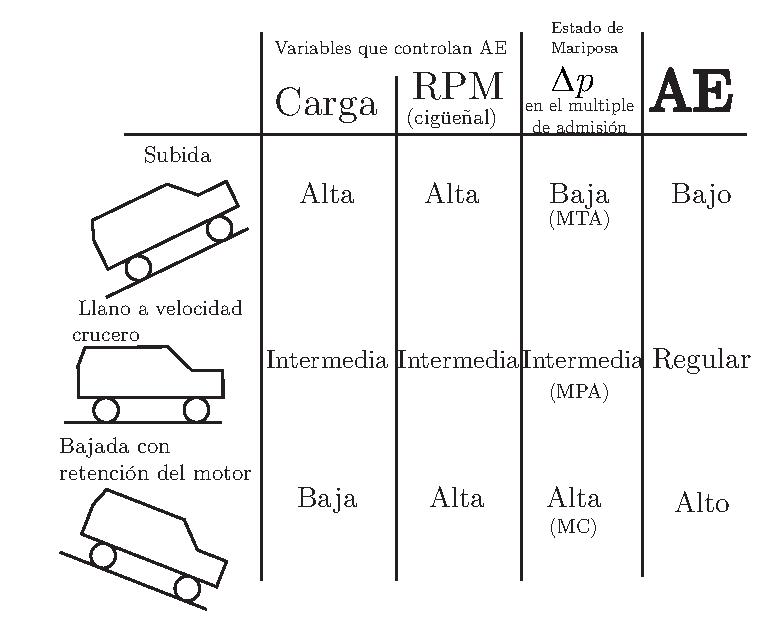
\includegraphics[width=0.49\textwidth]{fig/diag_auto.eps}
    \caption{Tabla de valores relevantes al AE.}
    \label{fig:AEmotor}
\end{figure}

\begin{figure}[htb!]
    \centering
    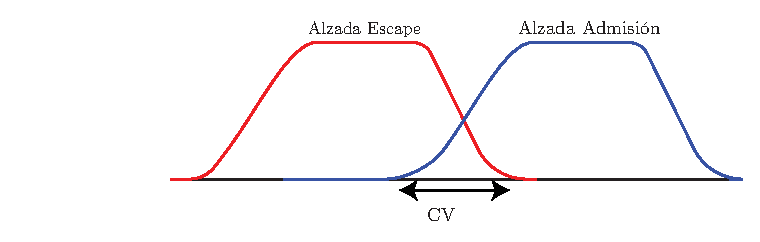
\includegraphics[width=0.49\textwidth]{fig/alzada.eps}
    \caption{Diagrama de alzada para un MCI.}
    \label{fig:alzadaMCI}
\end{figure}




\section{La detonación}
Se desea evitarla a todos costo. Sucede cuando una mezcla fresca explota antes que la alcance el frente de llama de la mezcla encendida(ignición controlada). Se puede evitar la detonación mediante el avance de encendido. Cabe destacar que si la mezcla se enciende antes de la chispa deja de ser detonación y pasa a ser llamado \textit{pre-ignición} o \textit{autoencendido}. En este ultimo proceso \textbf{no} participa la chispa del encendido. \textbf{Son dos procesos diferentes que ocurren en momentos distintos.}



